\chapter{Methodology} \label{sec:methodology}
This chapter describes the methodology used in this work, including the BERT baseline model, the feature fusion model architecture, the SHAP explainability analysis, and the analysis of misclassifications.
\section{Initial Chunking Strategy for BERT Fine-tuning}

The first preprocessing pipeline was developed to provide a straight BERT baseline for fine-tuning. Each conversation was reconstructed from the \textit{dialogue} field in the data into a single string with explicit speaker tags. Tokenization was then applied to the full conversation, with a maximum length of 512 tokens to provide the maximum information context in each chunk. Chunk boundaries could occur in the middle of a message. Conversations exceeding the 512 limit were split into non-overlapping chunks, which could occur at arbitrary positions within the text. Therefore, a single conversation could have multiple chunks, each treated as an independent training example. Finally, dynamic padding was applied at batch time and the tokenized dataset was then passed to the Hugging Face \textit{Trainer} for BERT fine-tuning without additional preprocessing steps.

%%%geändert 

\subsection{Train-Test Split}
For the finetuning, a train-test split was applied using \textit{GroupShuffleSplit} from \textit{sklearn}, ensuring, that all conversations from a single predator were contained completely in either the training or test set.  The split ratio was set to 70\% for training and 30\% for testing. Also, the same ratio of grooming to non-grooming conversations was kept in both sets to ensure balanced class distributions in the training and train and test data.

The resulting data distribution after chunking is shown in the following table.

\begin{table}[H] 
\label{tab:initial_split} 
\centering
\small
\caption[Initial data distribution after chunking]{\textbf{Initial data distribution after Chunking (max length 512, no message boundary control).}}
\begin{tabular}{lccc}
\hline
Split & Grooming & Non-Grooming PAN12  & \textbf{Total} \\
\hline
Train & 14997 & 30781  & \textbf{45778} \\
Test  & 1330 & 3429   & \textbf{4759} \\
\end{tabular}
\end{table}

%%%geändert

\section{BERT fine-tuning as Baseline}

Based on the initial chunking pipeline, BERT was fine-tuned for binary classification. 

The normal baseline followed a classic fine-tuning pipeline for binary classification with \textit{bert-base-uncased}. The training configuration was as follows:

\begin{itemize}
  \item \textbf{Backbone:} \textit{bert-base-uncased} (standard model dropouts)
  \item \textbf{Chunk length:} 512
  \item \textbf{Trainer/Optimization:} Hugging Face \textit{Trainer}
  \item \textbf{Epochs:} 3
  \item \textbf{Batch Size:} 8 
  \item \textbf{Learning Rate:} \textit{2e-5}
  \item \textbf{Weight Decay:} 0.01
  \item \textbf{Warmup:} none
  \item \textbf{Gradient Clipping:} not set
\end{itemize}



\subsection{Evaluation Metrics}
To evaluate the performance of the binary classifier, the most common metrics for a binary classification task were used in \textbf{all the following model evaluations}:

Let $TP$, $FP$, $TN$, and $FN$ be true positives, false positives, true negatives, and false negatives. 
The metrics are defined as follows:

\begin{align}
\text{Accuracy} &= \frac{TP + TN}{TP + TN + FP + FN}, \\
\text{Precision} &= \frac{TP}{TP + FP}, \\
\text{Recall} &= \frac{TP}{TP + FN}, \\
F_{1} &= 2 \cdot \frac{\text{Precision} \cdot \text{Recall}}{\text{Precision} + \text{Recall}}.
\end{align}

Therefore, Accuracy measures the proportion of correctly classified instances, while precision measures the proportion of predicted positive instances that are true positives. 
Recall measures the fraction of actual positive instances that are correctly identified, showing the model's ability to minimize false negatives. 
Finally, the $F_{1}$-score is reported as the harmonic mean of precision and recall, providing a balanced measure that accounts for both. 

Since the dataset is slightly imbalanced, the $F_{1}$-score for the positive class is used as the primary metric, ensuring that both precision and recall are equally considered for evaluation.

The evaluation was performed every 3000 steps during training, using the test dataset.

%%%geändert

\section{Limitations of Initial BERT Fine-tuning Approach}

\textbf{While the initial fine-tuning apporach enabled an effective baseline, it also included methodological concerns:}
\begin{enumerate}
  \item \textbf{Domain Leakage:} Since all PJ conversations have label 0 and all PAN12 conversations have label 1, the model could rely on dataset-specific artifacts (domain leakage) instead of semantic cues. As a result, the model might learn to distinguish between datasets rather than real grooming patterns.
  \item \textbf{Length Leakage:} In addition, PJ conversations are generally longer than the ones from PAN12 (Figure ~\ref{fig:conversation_word_lengths}), making conversation length a potential shortcut (length leakage). As a result, the model could exploit the length differences rather than learning real grooming-related features.
\end{enumerate}

\textbf{As shown later in the evaluation (Table ~\ref{tab:bert_base}), the initial model indeed achieved a very high performance, which motivated the design of a stricter preprocessing pipeline.} Therefore, a second preprocessing script was developed, which introduced fixed-length padding, enforced chunking at message boundaries, and included ynthetic non-grooming data in PJ style to reduce domain and length leakage. The following sections describe this improved pipeline in detail.

%% geändert
\section{Chunking Strategy for BERT to reduce Domain and Length Leakage}

To reduce leakage effects, a stricter preprocessing pipeline was implemented. Instead of splitting conversations at arbitrary positions, chunks were created only at message boundaries, ensuring that single utterances remained intact.

To further reduce domain leakage and length leakage, synthetic non-grooming chats in PJ style were added (Section~\ref{sec:synthetic-data}). Models were then trained and tested under the following two setups: 

\begin{enumerate}
  \item \textbf{Separated Split:} With synthetic data only in the test set, to probe generalization.
  \item \textbf{Mixed Split:} With synthetic data included in both train and test sets, to strengthen robustness.
\end{enumerate}


\subsection{Chunk-Length Distributions (For Train and Test) Across Sequence Lengths}\label{sec:chunk-length-distributions}

To determine the optimal chunk length for the BERT baseline, the mean, standard deviation, median, minimum, and maximum of tokens per conversation across the different datasets were calculated and are shown in table~\ref{tab:token_stats}. 

\begin{table}[htbp]
\centering
\caption{Token statistics per conversation/file across datasets}
\label{tab:token_stats}
\begin{tabular}{lrrrrrrr}
\toprule
\textbf{Dataset} & \textbf{Files} & \textbf{Mean} & \textbf{Std (pop)} & \textbf{Std (sample)} & \textbf{Median} & \textbf{Min} & \textbf{Max} \\
\midrule
PJ (grooming)                & 6\,175  & 723.83 & 446.54 & 446.58 & 719  & 12  & 1\,850 \\
PAN12                        & 27\,751 & 210.12 & 202.20 & 202.20 & 144  & 1   & 3\,656 \\
Synthetic                    & 621     & 969.47 & 161.24 & 161.37 & 972  & 488 & 1\,435 \\
PAN12 + Synthetic            & 28\,372 & 226.74 & 230.01 & 230.01 & 147  & 1   & 3\,656 \\
ALL (PJ + PAN12 + Synthetic) & 34\,547 & 315.59 & 339.65 & 339.65 & 171  & 1   & 3\,656 \\
\bottomrule
\end{tabular}
\end{table}

As again shown in table~\ref{tab:token_stats}, PJ conversations are much longer (mean: 724 tokens, median: 719 tokens) than PAN12 conversations (mean: 210 tokens, median: 144 tokens). The synthetic conversations are even longer (mean: 969 tokens, median: 972 tokens) and thus closer to the PJ distribution. The combined PAN12 + Synthetic dataset has a mean of 227 tokens and a median of 147 tokens, which is still much shorter than PJ. 
To evaluate the base model across these datasets, it was decided to test the baseline training with the following three fixed chunk sizes to evaluate, if the chunk size has an impact on performance and model robustness:
\begin{itemize}
  \item \textbf{150 tokens:} closely matches the PAN12 median while minimizing fragmentation for PAN12.
  \item \textbf{250 tokens:} offers additional context beyond the PAN12 median (covering a larger share of its distribution).
  \item \textbf{512 tokens:} contains full-length context for longer PJ/Synthetic conversations.
\end{itemize}

Consequently, the following three sequence lengths (150, 250, and 512) were generated, and padding on these fixed lengths was applied to test the impact of chunk size on performance, preventing the model from relying only on length differences between datasets.

%%%geändert

Figure~\ref{fig:chunk-dists} shows the resulting chunk length distributions for the three target lengths (150, 250, 512) after applying the improved chunking strategy, to show the impact of different chunk sizes on the dataset. Each subplot shows the distribution of chunk lengths in training and test sets combined. The orange bars represent grooming chunks collected from PJ, while the blue bars represent non-grooming chunks collected from PAN12. Additionally the green bars show the synthetic non-grooming chunks in PJ style. The Chunk lengths were measured before padding on a fixed size of 512, 250 or 150 chunks was applied.


\begin{figure}[H]
  \centering
  \begin{subfigure}[t]{0.34\textwidth}\centering
    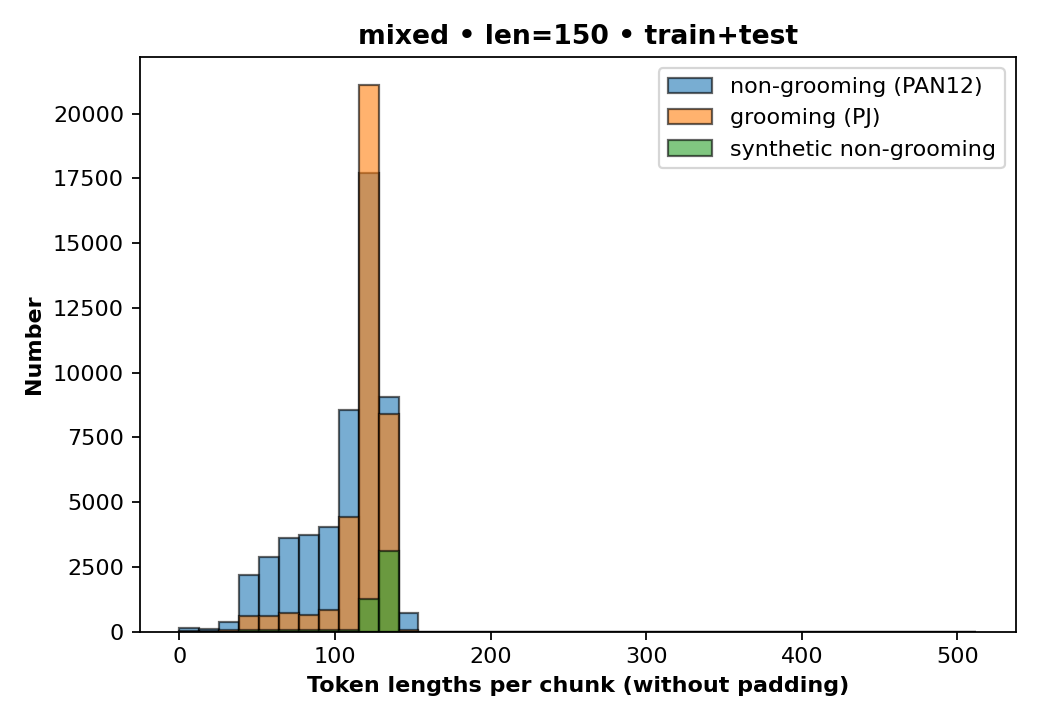
\includegraphics[width=\linewidth]{figures/chunkin_150_dist.png}
    \caption{150 tokens}\label{fig:chunkdist150}
  \end{subfigure}\hspace{-0.5em}% enger rücken
  \begin{subfigure}[t]{0.34\textwidth}\centering
    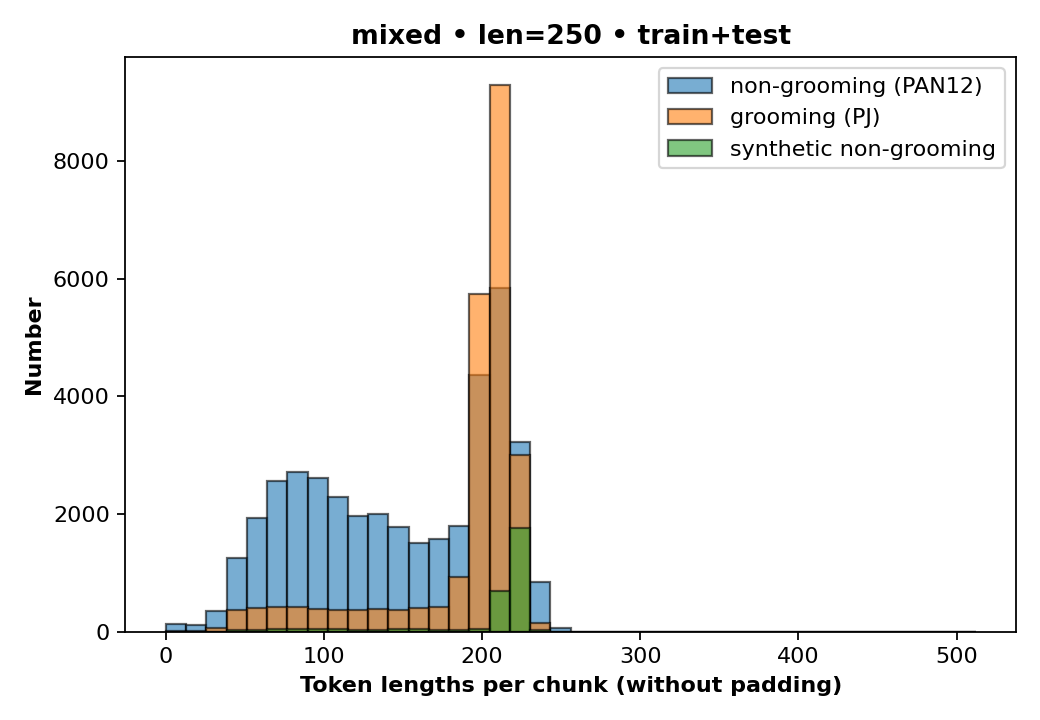
\includegraphics[width=\linewidth]{figures/chunking_250_dist.png}
    \caption{250 tokens}\label{fig:chunkdist250}
  \end{subfigure}\hspace{-0.5em}%
  \begin{subfigure}[t]{0.34\textwidth}\centering
    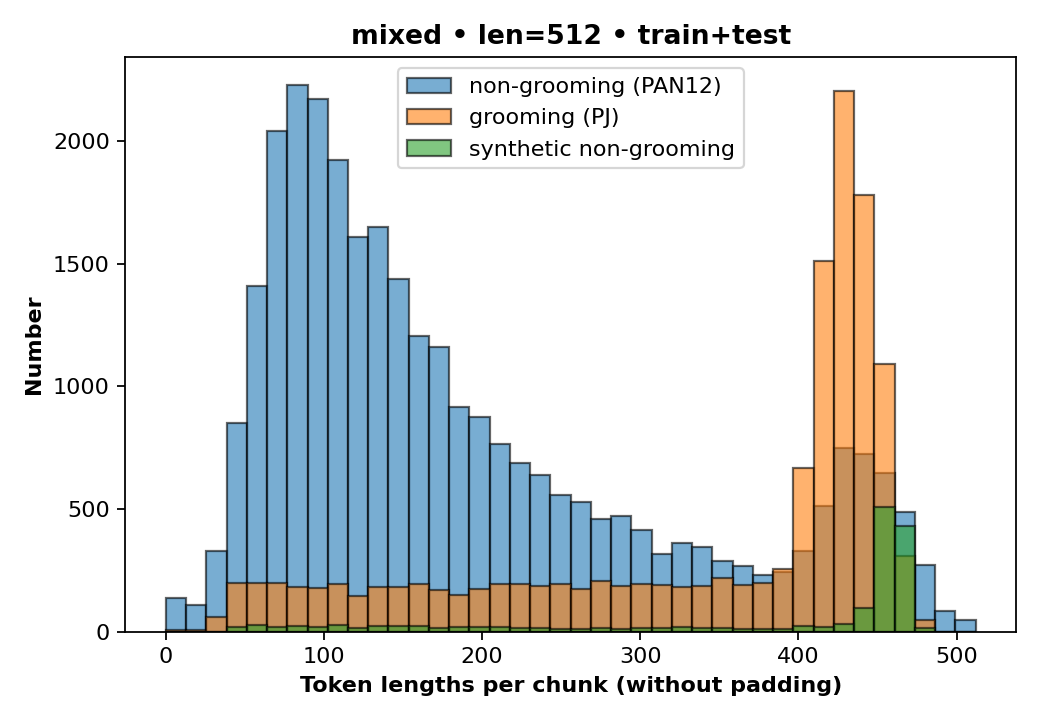
\includegraphics[width=\linewidth]{figures/chunking_512_dist.png}
    \caption{512 tokens}\label{fig:chunkdist512}
  \end{subfigure}
  \caption[Chunk Length Distributions]{Chunk length distributions (train+test) for different sequence lengths (before padding).}
  \label{fig:chunk-dists}
\end{figure}


\subsection{Data Distributions after Chunking}
 The following tables show the resulting data distributions after chunking for the three target lengths (150, 250, 512) and each setup (synthetic data only in test set and synthetic data in test and train set). Each table lists the number of chunks per class in the training and test sets for, together with the total number of chunks. 

 \begin{table}[H]
\centering
\small
\begin{tabular}{lcccc}
\hline
Split & Grooming & Non-Grooming PAN12 & Non-Grooming Synthetic & \textbf{Total} \\
\hline
Separated Train & 27883 & 36954 & 0    & \textbf{64837} \\
Separated Test  &  9625 & 16211 & 4749 & \textbf{30585} \\
\midrule[\heavyrulewidth]
Mixed Train     & 26583 & 37356 & 3254 & \textbf{67193} \\
Mixed Test      & 10925 & 15809 & 1495 & \textbf{28229} \\
\hline
\end{tabular}
\caption[Split for Chunk-Length of 150 Tokens]{\textbf{Split for Chunk-Length of 150 Tokens.}}
\end{table}


 \begin{table}[H]
\centering
\small
\begin{tabular}{lcccc}
\hline
Split & Grooming & Non-Grooming PAN12 & Non-Grooming Synthetic & \textbf{Total} \\
\hline
Separated Train & 17487 & 27057 & 0    & \textbf{44544} \\
Separated Test  &  6003 & 11848 & 2925 & \textbf{20776} \\
\midrule[\heavyrulewidth]
Mixed Train     & 16662 & 27321 & 2008 & \textbf{45991} \\
Mixed Test      &  6828 & 11584 & 917  & \textbf{19329} \\
\hline
\end{tabular}
\caption[Split for Chunk-Length of 250 Tokens]{\textbf{Split for Chunk-Length of 250 Tokens.}}
\end{table}


 \begin{table}[H]
\centering
\small
\begin{tabular}{lcccc}
\hline
Split & Grooming & Non-Grooming PAN12 & Non-Grooming Synthetic & \textbf{Total} \\
\hline
Separated Train & 9699 & 21259 & 0    & \textbf{30958} \\
Separated Test  & 3267 & 9195  & 1583 & \textbf{14045} \\
\midrule[\heavyrulewidth]
Mixed Train     & 9197 & 21352 & 1087 & \textbf{31636} \\
Mixed Test      & 3769 & 9102  & 496  & \textbf{13367} \\
\hline
\end{tabular}
\caption[Split for Chunk-Length of 512 Tokens]{\textbf{Split for Chunk-Length of 512 Tokens.}}
\end{table}



\section{Improved Training Pipeline} \label{sec:improved-training-pipeline}


For training on this improved dataset, the same BERT backbone was used but with a slightly more robust training configuration. Dropout rates in the classification head were increased (0.3), and label smoothing (0.1) was applied to reduce overconfidence. Gradient checkpointing was enabled for memory efficiency. 

\subsection{Improved Training Configuration}

The training configuration for the improved pipeline was the following:

\begin{itemize}
  \item \textbf{Backbone:} \textit{bert-base-uncased} with increased dropouts
  \item \textbf{Sequence length:} Variants \(\in \{150, 250, 512\}\) 
  \item \textbf{Dropout (BERT):} \(\textit{hidden\_dropout\_prob}=0.3\), \(\textit{attention\_probs\_dropout\_prob}=0.3\)
  \item \textbf{Loss function:} Cross-Entropy 
  \item \textbf{Label smoothing:} \(0.1\) 
  \item \textbf{Epochs:} \(3\)
  \item \textbf{Batch size:} \(8\)
  \item \textbf{Learning rate:} \(2\times10^{-5}\)
  \item \textbf{Weight Decay:} \(0.01\)
  \item \textbf{Warmup Ratio:} \(0.06\)
  \item \textbf{Max Grad Norm:} \(1.0\)
  \item \textbf{Gradient Checkpointing:} enabled 
\end{itemize}


\subsection{Evaluation Strategy with Additional Subsets}

The model was trained and tested across all three chunking target lengths (150, 250, 512) under two different setups
\begin{enumerate}
\item \textbf{Synthetic data only in the test set.}
This setup was designed to evaluate whether the model can generalize to PJ-style negatives without having seen them during training.
\item \textbf{Synthetic data in both train and test sets.}
This setup was designed to test if including synthetic non-grooming data in the training phase improves the model robustness and reduces reliance on dataset specific artifacts.
\end{enumerate}

The evaluation was again performed every 3000 steps on the test set, using accuracy, precision, recall, and F1 score as metrics. To further test the model robustness, an evaluation on only the synthetic data in the test set was performed. Here, only the accuracy was reported, since precision, recall, and F1 are not defined for a single class. Additionally the confusion matrix was calculated for the complete test set after each evaluation step to analyze the types of errors made by the model. Also, the ROC-Curve and the AUC score were calculated after each evaluation step to analyze the model's performance across different classification thresholds.

The detailed outcomes of the training across alle different chunk size and train/test split are shown in the evaluation section (Section~\ref{sec:bert_chunk_size_and_data_setup}).

\section{Choosing the final configuration for Feature Fusion and SHAP Explainability Analysis} 


Based on the evaluation across different chunk sizes and dataset configurations (Section \ref{sec:bert_chunk_size_and_data_setup}), \textbf{it was decided to continue the feature fusion and explainability analysis with a chunk size of 512 tokens in combination with the mixed split strategy having synthetic data in the train and test set}. Although shorter chunks were hypothesized to reduce length leakage, the results showed no significant performance decline for 150 or 250 tokens. 512-token chunks consistently achieved the best F1 scores (up to 0.97) while at the same time providing richer conversational context, which is crucial for a clean LIWC analysis. Moreover, having the synthetic data only in the test set revealed a poor generalization. In comparison, the mixed split setup led to a more robust performance across all evaluation subsets, making it the more reliable and realistic configuration for further experiments, setting a stable foundation for the following feature fusion and SHAP analysis.

%%%geändert

\section{Choosing the LIWC Feature Set for Feature Fusion and SHAP Explainability Analysis} \label{sec:liwc-feature-selection}

%% überarbeitet


\textbf{The Feature Fusion and following SHAP explainability analysis was performed with two variants of feature sets in each case: }
\begin{enumerate}
    \item \textbf{All-Features-Fusion}: Use of all 118 LIWC features.
    \item \textbf{Psychometric-Fusion}: Use of a subset of \textbf{49 psychometric LIWC features} coverings all psycholinguistic LIWC features that are highlighted in the literature as relevant for manipulative communication in Grooming Chats (Section \ref{psychometric_liwc_features_in_grooming}). The subset contains the following categories and dimensions:
\end{enumerate}

\subsubsection{Psychometric LIWC Subset (49 features)}

\begin{itemize}
  \item \textbf{Drives}: \textit{Affiliation}, \textit{Achievement}, \textit{Power}, \textit{Reward}, \textit{Risk}, \textit{Curiosity}, \textit{Allure}
  \item \textbf{Cognition}: \textit{All-or-none}, \textit{Cognitive Processes}, \textit{Insight}, \textit{Causation}, \textit{Discrepancy}, \textit{Tentative}, \textit{Certitude}, \textit{Differentiation}, \textit{Memory}
  \item \textbf{Affect \& Emotion}: \textit{Affect}, \textit{Positive Tone}, \textit{Negative Tone}, \textit{Emotion}, \textit{Positive Emotion}, \textit{Negative Emotion}, \textit{Anxiety}, \textit{Anger}, \textit{Sadness}, \textit{Swear Words}
  \item \textbf{Social}: \textit{Social Behavior}, \textit{Prosocial Behavior}, \textit{Politeness}, \textit{Interpersonal Conflict}, \textit{Moralization}, \textit{Communication}, \textit{Social Referents}, \textit{Family}, \textit{Friends}, \textit{Female References}, \textit{Male References}
  \item \textbf{Physical}: \textit{Health}, \textit{Illness}, \textit{Wellness}, \textit{Mental Health}, \textit{Substances}, \textit{Sexual}, \textit{Food}, \textit{Death}
\end{itemize}


This subset was designed to isolate psychologically interpretable features from LIWC. The corresponding group features(for example \textit{Cognition}, \textit{Affect}, \textit{Social}) were retained not only because they are automatically computed together with their subset categories, but also provide meaningful aggregation levels, which allows to identify, which broader psychological domains (for example cognitive versus affective language) contribute most strongly to the model's descision, even when individual subcategories show smaller or inconsistent effects. 

In contrast, the \textbf{summary variables} like \textit{Tone}, \textit{Analytic}, \textit{Clout}, and \textit{Authentic} were excluded from the psychometric subset. These dimensions primarily reflect \textit{stylistic and structural} characteristics of language rather than \textit{psychometric} content~\cite{pennebaker2022liwc,tausczik2010psychological}. 
Their exclusion ensures that the subset focuses on psychologically meaningful word categories, rather than composite style based indicators. 


\section{LIWC Data Extraction}
The LIWC features were extracted using the official LIWC-22 software. The extraction was done once over complete PJ and PAN12 conversations, as well as the synthetic non-grooming conversations in PJ style. Furthermore, the LIWC features were also extracted for each chunk in the improved chunked dataset with a chunk size of 512 tokens(Section \ref{sec:methodology}).

Also, the LIWC Features were extracted in two variants: once with all 118 features and once with the psychometric subset of 49 features (Section \ref{sec:liwc-feature-selection}). The extracted LIWC features were then stored in a separate sidecar file.

\section{LIWC Data Analysis}

In order to analyze the effect size of LIWC features prior to fine-tuning, an analysis of LIWC features across all conversations was performed.
The LIWC-based analysis was carried out in two steps. First, a global comparison was performed on complete conversations, followed by a chunk-based comparison using 512 chunks, which was used in the following feature fusion. Both analyses were performed once for the complete set of LIWC-2022 features and once restricted to the psychometric subset of LIWC features to determine if psychometric variables alone are sufficient to distinguish grooming conversations from non-grooming conversations.

%%geändert 

\subsection{Global LIWC Analysis on Complete Conversations}

For the global analysis, all grooming conversations from the PJ were first aggregated into one conversation per groomer to represent their general language style, while non-grooming conversations from PAN12 were used in their original form. 
For each conversation, the complete set of LIWC-2022 features was calculated.  
To improve interpretability, the features were grouped into their macro categories according to the LIWC-2022 manual:

\begin{itemize}
    \item \textbf{Linguistic:} Function words, Pronouns, Personal pronouns, First person singular, First person plural, Second person, Third person singular, Third person plural, Impersonal pronouns, Determiners, Articles, Numbers, Prepositions, Auxiliary verbs, Adverbs, Conjunctions, Negations, Common verbs, Common adjectives, Quantities
    \item \textbf{Punctuation:} Periods, Commas, Question marks, Exclamation marks, Apostrophes, Other punctuation
    \item \textbf{Emoji:} Emojis
    \item \textbf{Drives:} Affiliation, Achievement, Power
    \item \textbf{Motivation:} Reward, Risk, Curiosity, Allure
    \item \textbf{Cognition:} Cognitive processes, All-or-none, Insight, Causation, Discrepancy, Tentativeness, Certitude, Differentiation, Memory
    \item \textbf{Affect:} Positive tone, Negative tone, Emotion, Positive emotion, Negative emotion, Anxiety, Anger, Sadness, Swear words
    \item \textbf{Social:} Social behavior, Prosocial behavior, Politeness, Interpersonal conflict, Moralization, Communication, Social referents, Family, Friends, Female references, Male references, Social processes
    \item \textbf{Physical:} Health, Illness, Well Being, Mental health, Substances, Sexual, Food, Death, Physical processes
    \item \textbf{Perception:} Attention, Motion, Space, Visual perception, Auditory perception, Feeling (perceptual)
    \item \textbf{Culture:} Politics, Ethnicity, Technology
    \item \textbf{States:} Need, Want, Acquire, Lack, Fulfilled, Fatigue
    \item \textbf{Time:} Time, Past focus, Present focus, Future focus
    \item \textbf{Conversation:} Netspeak, Assent, Nonfluencies, Fillers
\end{itemize}


For each conversation, the value of a macro group was defined as the arithmetic mean of all available member feature values. Then, the macro group means were averaged across all conversations for each class (PJ vs. PAN12). 
The results were visualized as grouped bar charts (PJ vs. PAN12) sorted by the overall mean \(\tfrac{1}{2}(\overline{g}_{\mathrm{PJ}}+\overline{g}_{\mathrm{PAN}})\) .

In addition to macro group aggregation, each individual LIWC feature was statistically analyzed. For each feature \(f\), the mean and standard deviation across all conversations were calculated per class,
\[
\overline{x}_{\mathrm{PJ}},\ s_{\mathrm{PJ}},
\qquad
\overline{x}_{\mathrm{PAN}},\ s_{\mathrm{PAN}},
\]
followed by the mean difference \(\Delta = \overline{x}_{\mathrm{PJ}} - \overline{x}_{\mathrm{PAN}}\) and Cohen's \(d\)~\cite{cohen1988},
\[
d = \frac{\Delta}{s_p},
\qquad
s_p = \sqrt{\frac{(n_{\mathrm{PJ}}-1)s_{\mathrm{PJ}}^2+(n_{\mathrm{PAN}}-1)s_{\mathrm{PAN}}^2}{n_{\mathrm{PJ}}+n_{\mathrm{PAN}}-2}}.
\]

The descriptive statistics and effect sizes were written into a summary table for all LIWC features which is provided in the appendix (table \ref{tab:liwc22-categories}).

Furthermore, the 30 LIWC-2022 features with the largest absolute effect sizes \(|d|\) were selected to identify the most discriminative variables. For this comparison, Cohen’s \(d\) was computed for each feature, and the 30 features with the largest absolute effect sizes \(d\) were visualized as horizontal bar plots to identify the most discriminative linguistic variables. To ensure methodological consistency and to further evaluate the \textbf{quality and representativeness of the synthetically generated non-grooming data}, the same analysis was applied to compare the synthetic dataset separately with the \textbf{PJ-grooming} and \textbf{PAN12-non-grooming} data. This step was intended to identify potential linguistic deviations between the synthetic and real-world data and to evaluate if the synthetic data exhibits similar patterns as PAN12.


The results of the global LIWC analysis are presented in the evaluation section (Section~\ref{sec:global_liwc_analysis}).

\subsection{Chunk-based LIWC Analysis with 512 Tokens}

To analyse the patterns within the conversation segments used for the feature fusion training, a chunk-based analysis was performed with a fixed chunk size of 512 tokens. For each chunk, a LIWC-2022 feature vector was calculated, and the average values per class were determined across all chunks. 
For each feature, the range
\[
\mathrm{range}(f) = \max_{s}\overline{f}_{s} - \min_{s}\overline{f}_ {s}
\]
was determined across all sources (\(s \in \{\mathrm{PJ}, \mathrm{PAN12}, \mathrm{SYN}\}\)), and the top 15 features, again based on Cohen's \(d\)~\cite{cohen1988} with the largest ranges between the PJ and PAN12 data were selected for visualization. This was done since PJ and PAN12 together comprise the majority of the training corpus (>\,80\%) and the analysis should focus more on the real data.
The visualization and evaluation of the chunk-based LIWC analysis is presented in section~\ref{sec:chunk_based_liwc_analysis}.

\section{Feature Fusion Strategy}

%%Überarbeiter

To extend the BERT baseline with the additional input of LIWC features, the LIWC features were first extracted chunk-wise and stored as numerical vectors in a separate sidecar file. This sidecar contained a key consisting of \textit{chunk\_index} (for dialogues consisting of several chunks) and  \textit{conv\_id}, as well as the corresponding chunk-specific LIWC features. 
When loading the dataset, the sidecar files were assigned to the respective chunks based on the \textit{conv\_id} and the \textit{chunk\_index}, so that the training and test data sets contained a column for \textit{liwc} in addition to \textit{input\_ids}, \textit{attention\_mask}, and \textit{labels}. 

To integrate the LIWC features into the BERT architecture, \textbf{a late fusion approach} was implemented using cross-attention and a gating mechanism. This method allowed the model to select information from LIWC into the contextualized token representations learned by BERT. 

%%%geändert

\subsection{Model Architecture}

The proposed feature fusion model extends \textit{bert-base-uncased} (12 transformer layers, hidden size \(d_h=768\), 12 attention heads) with a late-fusion mechanism that integrates LIWC features into the transformer encoder in the upper encoder layers at \textbf{layer 6 and 12}. The design was used to keep the original BERT architecture and its pre-trained weights intact while allowing the model to leverage additional information from LIWC. This keeps the tokenization and main contextual processing of the text unchanged, while the LIWC information is  introduced after language modeling, which holds comparability with the BERT baseline and allows a later downstream explainability using SHAP. The overall process can be summarized as follows:

\begin{itemize}
    \item \textbf{Input and Feature Projection:}
    \begin{itemize}
        \item For each text chunk, a LIWC feature vector \(x \in \mathbb{R}^{d_{liwc}}\) is extracted \(d_{liwc}=118\) for all features or \(d_{liwc}=49\) for the psychometric subset).
        \item \(x\) is normalized using \textit{LayerNorm} and mapped through a linear projection with \textit{GELU} activation to a compact fusion dimension \(z \in \mathbb{R}^{d_p}\) (\textit{proj\_dim}, (for example 128/768).
        \item From \(z\), a single \emph{LIWC token} \(t \in \mathbb{R}^{d_h}\) is generated via a linear layer. This token summarizes the LIWC information for the entire chunk.
    \end{itemize}

    
    \item \textbf{Fusion via Cross-Attention:}
    \begin{itemize}
        \item Text hidden states \(H \in \mathbb{R}^{T \times d_h}\) from intermediate layers serve as \textbf{queries}.
        \item The LIWC token \(t\) is used as \textbf{key/value} in a multi-head cross-attention mechanism (\textit{n\_heads}=4, mask-aware).
        \item This enables each token to attend to the psycholinguistic context selectively.
    \end{itemize}
    
    \item \textbf{Gating and Residual Update:}
    \begin{itemize}
        \item A channel-wise gate \(g \in \mathbb{R}^{d_h}\) (\textit{gate\_type}=\textit{channel}) is computed from the \textit{[CLS]} representation and \(z\).
        \item The final representation is updated via \[H' = H + g \odot \mathrm{Attn}(H, t)\] followed by a 10\% dropout.
        \item A post-fusion \textit{LayerNorm} is applied to stabilize training and normalize the residual update.

    \end{itemize}
    
    \item \textbf{Integration in Encoder:}
    \begin{itemize}
        \item The fusion block is applied in the encoder layers (layers 6 and 12) \textit{fusion\_at\_layers} with \textit{depth}=1).
        \item After the final fusion layer, the \textit{[CLS]} vector is pooled as in the baseline model and passed to a linear classification head.
        \item The pooled \textit{[CLS]} representations are combined by averaging (\textit{mean}). The resulting fused representation is then passed to the linear classifier.

    \end{itemize}
\end{itemize}
    
%%%geändert

The overall feature fusion architecture is illustrated in the following figure~\ref{fig:liwc-bert-fusion}.

\begin{figure}[H]
    \centering
    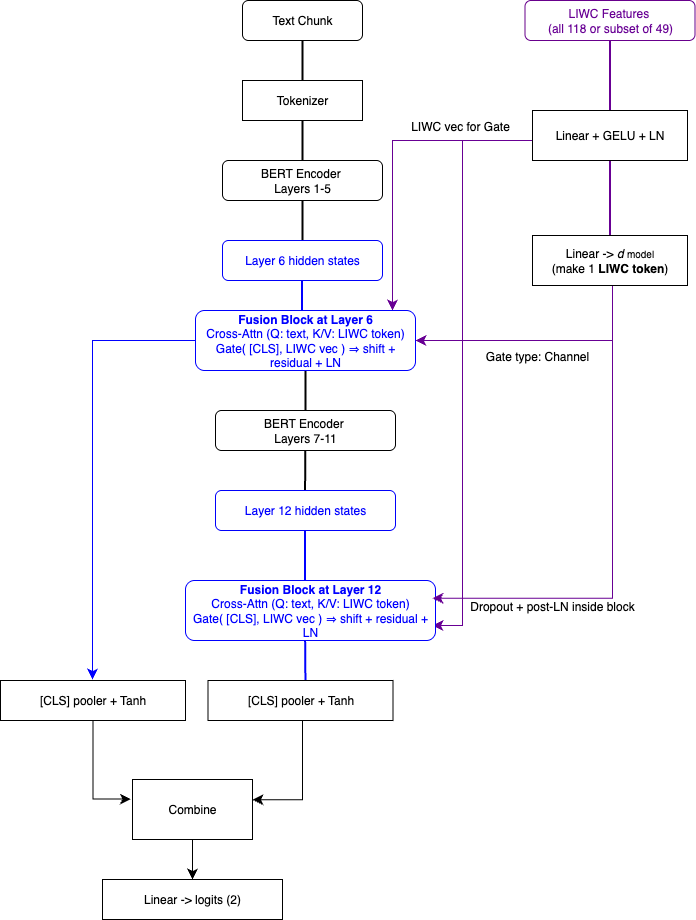
\includegraphics[width=0.7\textwidth]{new_fusion.png}
    \caption[Feature Fusion Architecture]{Late fusion of LIWC with BERT: LIWC features (either all 118 or the 49 psychometric subset) are projected, transformed into a single \emph{LIWC token}, and fused with hidden states from layers 6 and 12 with cross-attention plus a gating mechanism (Multimodal Shifting). The resulting fusion blocks are applied in parallel to the BERT encoder and do not feed back into subsequent layers. The [CLS] representations from both fusion points are pooled, combined, and classified. The \textcolor{blue!70!black}{blue blocks} highlight where fusion takes place, while the \textcolor{violet!70!black}{purple line} represents the LIWC stream (projection and token).}
\label{fig:liwc-bert-fusion}

\end{figure}

\subsection{Training Pipeline and Evaluation}

The training and evaluation of the feature fusion model followed a similar pipeline as the improved BERT-Baseline (Section~\ref{sec:improved-training-pipeline}). With the following hyperparameters:

\begin{itemize}
\item \textbf{Number of Epochs:} \(3\) 
\item \textbf{Saving Checkpoint at Epoch:}\(1\) 
\item \textbf{Evaluation Steps:} \(3000\)
\item \textbf{Learning Rate:} \(2\times10^{-5}\)
\item \textbf{Weight Decay:} \(0.01\)
\item \textbf{Warmup Ratio:} \(0.06\)
\item \textbf{Max Grad Norm:} \(1.0\)
\item \textbf{Batch Size:} \(8\)
\item \textbf{Loss Function:} Cross-Entropy with Label Smoothing of \(0.1\)
\item \textbf{Dropout inside Fusion} \(0.1\)
\item \textbf{Number of Heads in Cross-Attention:} \(4\)
\item \textbf{Fusion Depth:} \(1\)
\end{itemize}

The Evaluation was performed with the same metrics as in the BERT-Baseline (accuracy, precision, recall, balanced F1) and on the dataset with chunks consisting of 512 tokens and synthetic data in both train and test set. The evaluation was done every 3000 steps of training and the model was stored after each epoch.

\section{Explainability Analysis based on Feature Fusion Model}
To analyze the model's decision-making process, SHAP was used to show insights into how token-level text features and LIWC features contributed to the model's predictions. The fixed length LIWC vector calculated for each chunk served as input for the analysis. The following sections describe the two complementary explainability analyses that were performed. 
%%geändert

\subsubsection{Reducing Computational Costs with KernelSHAP}

The explanations were generated using KernelSHAP, where the text input of the model was capped to a fixed sequence length of \texttt{64} tokens. To keep the computational costs of the SHAP analysis manageable, a fixed configuration was used for the complete LIWC feature sets.  \texttt{3000} random samples from the test set were selected for explanation. To mitigate class-imbalance bias, all global statistics were computed on a \textbf{class-balanced subset} of the test set (50\% grooming, 50\% non-grooming). For the background distribution, \texttt{32} LIWC vectors were chosen and reduced to at most 20 representative centroids using k-means clustering. Each instance was then perturbed \texttt{256} times in order to approximate the marginal feature contributions. The model was executed in mini batches of \textit{4} explanations, with a maximum of \textit{16} perturbations processed in parallel. Additionally, the inference was carried out in mixed precision with disabled gradients and kept constant for all explanations. This reduced GPU memory consumption and made it feasible to perform KernelSHAP for both feature sets without exceeding hardware limits.

%%geändert

\subsubsection{Partitioning overall contribution into tokens vs.\ LIWC}\label{sec:token_vs_liwc_share}

To quantify the relative contribution of text tokens versus LIWC features to the model's decisions, two complementary attribution procedures were computed on the same set of explained instances and subsequently paired.

\subsubsection{Token-side attribution (Integrated Gradients)}

For each instance, token-level attributions were obtained with Integrated Gradients on the embedding input.
A zero embedding served as baseline, and attributions were computed with regard to the model's predicted class.
Let $a_{n,t}\in\mathbb{R}^d$ denote the IG vector for token $t$ in instance $n$ (embedding dimension $d$).
A scalar saliency per token was formed via the $\ell_2$ norm and aggregated across tokens to give a per-instance token total:
\[
S^{\mathrm{tok}}_{n}
\;=\;
\sum_{t} \lVert a_{n,t}\rVert_2.
\]
During Integrated Gradients, the LIWC branch was held fixed to a constant vector (median over the sidecar features) to avoid confounding text and LIWC effects.

\subsubsection{LIWC-side attribution (KernelSHAP)}

For the same instances, LIWC attributions was computed with KernelSHAP by varying the LIWC feature vector while keeping the text input fixed to a short sequence.
Let $\phi_{n,f}$ denote the SHAP value of LIWC feature $f$ for instance $n$.
Per-instance LIWC totals were formed by summing absolute SHAP values across features:
\[
S^{\mathrm{liwc}}_{n}
\;=\;
\sum_{f=1}^{F} \lvert \phi_{n,f}\rvert .
\]

Because the classifier has two output classes, KernelSHAP returns one attribution per class. Therefore class-agnostic attributions were used by averaging the absolute SHAP values across classes for each instance and feature before aggregation.

\subsubsection{Pairing and normalization}

For each explained instance \(n\), the two totals were combined into percentage shares:
\[
\mathrm{Share}^{\mathrm{liwc}}_{n}
\;=\;
\frac{S^{\mathrm{liwc}}_{n}}{S^{\mathrm{liwc}}_{n}+S^{\mathrm{tok}}_{n}}
\;\times\;100\%,
\qquad
\mathrm{Share}^{\mathrm{tok}}_{n}
\;=\;
\frac{S^{\mathrm{tok}}_{n}}{S^{\mathrm{liwc}}_{n}+S^{\mathrm{tok}}_{n}}
\;\times\;100\% .
\]
Global summaries were reported as the mean and median of these per-instance percentages over 3000 randomly sampled test instances.

%%%geändert

\subsubsection{Global importance of LIWC features}

For each LIWC feature $i$, the contribution over the balanced subset was aggregated with the \textbf{mean absolute} SHAP value, $\mathrm{mean}|\mathrm{SHAP}|_i$, and reported as normalized percentages for readability:
\[
\text{FeatureImportance}_{i}
= \frac{\mathrm{mean}\,|\mathrm{SHAP}|_{i}}{\sum_{j=1}^{F} \mathrm{mean}\,|\mathrm{SHAP}|_{j}} \times 100\% ,
\]
where $F$ is the number of LIWC features. This quantifies the share of the model’s decision attributable to feature $i$.

Based on the global Importance, the commulative importance of every LIWC features was determined by sorting the features descendingly and calculating the cumulative sum of the importance values. 
%%geändert

\subsubsection{Direction of Effect}

\textbf{Signed} SHAP values according to the grooming logit indicate direction:
\[
\mathrm{SHAP}^{(+)}_{i} > 0 \;\Rightarrow\; \text{feature } i \text{ pushes the prediction toward grooming,}
\]
\[
\mathrm{SHAP}^{(+)}_{i} < 0 \;\Rightarrow\; \text{feature } i \text{ pushes the prediction toward non-grooming.}
\]

\subsection{Confidence Analysis based on Label Flip and Confidence Shift}

To further analyze the impact of LIWC features on model decisions, model confidence and class assignment were calculated once with the regular LIWC feature vectors (\emph{LIWC on}) and once with LIWC vectors set to zero (\emph{LIWC off}). This allowed the influence of the additional LIWC features on model confidence and class assignment to be analyzed.

For both conditions, the class probability was determined by applying the softmax function to the logits. The highest probability \(p_{\max}\) represents the model confidence for the predicted class:
\[
p_{\max}^{(\text{on})} = \max_k p_k^{(\text{LIWC on})}, \qquad
p_{\max}^{(\text{off})} = \max_k p_k^{(\text{LIWC off})}.
\]

The difference between these two values defines the so-called \textbf{confidence shift}:
\[
\Delta p_{\max} = p_{\max}^{(\text{on})} - p_{\max}^{(\text{off})}.
\]
A positive value indicates that the LIWC features increased the certainty of the model decision, while a negative value describes a decrease in confidence.

In addition, it was analyzed, if the predicted class of an input changed as a result of LIWC fusion (for example, model decision = grooming before and model decision = non-grooming after). If such a change occurs, it is referred to as a \textbf{label flip}:
\[
\text{flip} = \mathds{1}\!\left[\,\hat{y}^{(\text{on})} \neq \hat{y}^{(\text{off})}\,\right], 
\qquad
\hat{y} = \arg\max_k p_k.
\]
The number and rate of label flips show the extent to which the LIWC features lead to a changed classification decision.

For quantitative analysis, the following metrics were calculated:
\begin{itemize}
    \item $\Delta \mu$, $\Delta \tilde{x}$, $\Delta \sigma$: Mean, median, and standard deviation of \(\Delta p_{\max}\).
    \item $\Delta p_{10}$, $\Delta p_{90}$: 10th and 90th percentiles of the distribution of \(\Delta p_{\max}\).
    \item $n_{\text{class 0}}$, $n_{\text{class 1}}$: Frequency distribution of the predicted classes with LIWC.
    \item $n_{\text{flips}}$, flip rate: Number and relative frequency of prediction changes.
\end{itemize}


The results are presented in Section ~\ref{sec:confidence_and_label_flip_analysis}.

\section{LIWC Analysis of Misclassifications}

To identify potential patterns in the misclassifications made by the feature fusion model, a LIWC analysis of false positives and false negatives was conducted. It was tested whether misclassified samples resemble the opposite correct class in LIWC space, for example, whether false negatives are closer to true negatives and false positives are closer to true positives according to their LIWC Feature values. Furthermore, it was analyzed which LIWC features differ significantly between misclassified and correctly classified samples. This analysis was again conducted with both the full LIWC feature set and the psychometric subset. The same fusion model, tokenizer, and LIWC sidecar vectors as in the previous sections were used to generate predictions and per-sample LIWC vectors. The analysis was performed on the complete test set.

\subsection{Per-feature group comparisons}
Per-feature comparisons were run for four group pairs: FP vs.\ TN, FN vs.\ TP, TN vs.\ FN, and TP vs.\ FP. For each LIWC feature \(f\), let \(x\) denote values in the first named group and \(y\) in the second. The following statistics were computed:

\begin{itemize}
\item \textbf{Mean difference:} \(\Delta\mu = \bar{x} - \bar{y}\).
\item \textbf{Again, Cohen's \(d\)  was used to quantify effect size}
\item \textbf{Significance tests:} The Mann–Whitney \(U\) test~\cite{mannwhithneyu1947} (two-sided) was used to assess the significance of differences in distributions of FP/TN and FN/TP.
\item \textbf{Multiple testing control:} The Benjamini–Hochberg procedure~\cite{benjaminhochberg} was applied across features to obtain FDR-adjusted \(q\)-values. For plotting, a significance score \(-\log_{10}(q)\) was used.
\end{itemize}

\subsection{Proximity hypothesis tests in LIWC feature space}
To test if the misclassifications by the fusion modek resemble the opposite correct group in LIWC space, distances were computed in a standardized feature space (z-scored per LIWC dimension). Let \(\mathbf{c}_{\mathrm{TN}}\) and \(\mathbf{c}_{\mathrm{TP}}\) be the centroids of TN and TP. For each FN sample with standardized vector \(\mathbf{z}\), Euclidean distances
\(d_{\mathrm{TN}} = \|\mathbf{z}-\mathbf{c}_{\mathrm{TN}}\|_2\) and
\(d_{\mathrm{TP}} = \|\mathbf{z}-\mathbf{c}_{\mathrm{TP}}\|_2\) were computed and the following one-sided hypotheses were tested:
\[
H_{1}^{\mathrm{FN}}:\; \Pr\!\big[d_{\mathrm{TN}} < d_{\mathrm{TP}}\big] > 0.5
\quad\text{and}\quad
H_{1}^{\mathrm{FP}}:\; \Pr\!\big[d_{\mathrm{TP}} < d_{\mathrm{TN}}\big] > 0.5.
\]
For each hypothesis, the analysis reported:

\begin{itemize}
  \item \textbf{Proportion of samples} closer to the hypothesized centroid:
  \[\hat{p} = \frac{1}{n} \sum_{i=1}^{n} \mathds{1}[d_{\text{closer}} < d_{\text{farther}}].\]
  \item \textbf{One-sided binomial test} against \(0.5\) to determine if the observed proportion \(\hat{p}\) is significantly greater than chance.
  \item \textbf{Paired one-sided tests} on the distance differences \(d_{\mathrm{TN}} - d_{\mathrm{TP}}\) for FN and \(d_{\mathrm{TP}} - d_{\mathrm{TN}}\) for FP. The Wilcoxon signed-rank test and the one-sample \(t\)-test were used to determine whether the mean and median difference is significantly greater than 0.
\end{itemize}

The results of the LIWC analysis of misclassifications are presented in section \ref{sec:misclassification_analysis}.

\subsection{SHAP-Based Proximity Analysis of Top-20 Misclassifications}

For a deeper analysis of misclassifications, an evaluation was performed based on the \textbf{top 20 LIWC features}, which were identified in Section~\ref{sec:global_ranking_top20} as the most relevant for the model's decision using the global importance SHAP values. This allowed to examine whether misclassifications can be explained by their proximity to the opposite correct class along these top LIWC dimensions. Also, focusing on the 20 most important features reduced the noise from less informative variables and enabled a more targeted analysis of group differences.

\subsubsection{Top-20 selection and SHAP direction}

All LIWC-2022 features were globally ranked by their \emph{mean\_abs} SHAP values, and the top 20 were selected. In addition, the SHAP sign (\emph{mean\_signed}) was used for each feature to define the “TP-like” versus “TN-like” direction.

\subsubsection{Z-scaling and SHAP-oriented projection}

To ensure comparability, feature columns were $z$-scaled. Each LIWC feature was then \emph{projected} onto the SHAP direction by multiplying, per sample, with the sign of its \emph{per-class SHAP margin}.  

For example \ $\operatorname{sign}(\Delta\mathrm{SHAP}_i)$ with
$\Delta\mathrm{SHAP}_i = \mathrm{SHAP}^{(+)}_i - \mathrm{SHAP}^{(-)}_i$ (grooming = $+$, non-grooming = $-$ and default class indices 1 and 0). 

On this aligned axis, values to the right of $x=0$ indicate greater similarity to true positives (TP-like), and values to the left indicate greater similarity to true negatives (TN-like). In both cases, multiplying $z$-scaled feature values by this sign yields a SHAP-aligned axis where values $>0$ are TP-like and values $<0$ are TN-like.

%%%geändert

\subsubsection{Group statistics and confidence intervals}

For each group $\{\mathrm{TP}, \mathrm{TN}, \mathrm{FP}, \mathrm{FN}\}$ and each top-$K$ feature, group means $\bar{x}$, standard deviations $s$, and standard errors
\[
SE \;=\; \frac{s}{\sqrt{n}}
\]
with $n$ as the group size were calculated on the projected values. For the misclassification groups (FP and FN), a 95\% confidence interval was computed as
\[
\mathrm{CI}_{95} \;=\; \bar{x} \pm 1.96 \cdot SE.
\]
The position of this interval relative to $x=0$ was classified as:
\emph{CI TP-side} (entirely $>0$), \emph{CI TN-side} (entirely $<0$), or \emph{CI crosses-0} (ambiguous).

\subsubsection{Proximity rate (TP/TN closeness)}

To determine whether misclassifications align more with TP or TN, per feature the absolute distances on the projected axis were compared:
\[
d_{\mathrm{FP}\to\mathrm{TP}} \;=\; \bigl|\bar{x}_{\mathrm{FP}} - \bar{x}_{\mathrm{TP}}\bigr|,\quad
d_{\mathrm{FP}\to\mathrm{TN}} \;=\; \bigl|\bar{x}_{\mathrm{FP}} - \bar{x}_{\mathrm{TN}}\bigr|,
\]
and analogously for FN. A feature is counted as “FP closer to TP” if $d_{\mathrm{FP}\to\mathrm{TP}} < d_{\mathrm{FP}\to\mathrm{TN}}$, and as “FN closer to TN” if $d_{\mathrm{FN}\to\mathrm{TN}} < d_{\mathrm{FN}\to\mathrm{TP}}$. Summary rates are reported over the top 20 features. 

The results of this analysis, including visualization and summary tables, are presented in Section~\ref{sec:shap_missclassification_analysis}.


